%% LyX 2.0.2 created this file.  For more info, see http://www.lyx.org/.
%% Do not edit unless you really know what you are doing.
\documentclass[british,english]{article}
\usepackage{utopia}
\usepackage{helvet}
\usepackage{courier}
\renewcommand{\familydefault}{\rmdefault}
\usepackage[T1]{fontenc}
\usepackage[latin9]{inputenc}
\usepackage{listings}
\usepackage[a4paper]{geometry}
\geometry{verbose,tmargin=2cm,lmargin=2cm,footskip=2cm}
\setlength{\parskip}{\bigskipamount}
\setlength{\parindent}{0pt}
\usepackage{array}
\usepackage{longtable}
\usepackage{refstyle}
\usepackage{graphicx}

\makeatletter

%%%%%%%%%%%%%%%%%%%%%%%%%%%%%% LyX specific LaTeX commands.

\AtBeginDocument{\providecommand\subref[1]{\ref{sub:#1}}}
%% Because html converters don't know tabularnewline
\providecommand{\tabularnewline}{\\}
\RS@ifundefined{subref}
  {\def\RSsubtxt{section~}\newref{sub}{name = \RSsubtxt}}
  {}
\RS@ifundefined{thmref}
  {\def\RSthmtxt{theorem~}\newref{thm}{name = \RSthmtxt}}
  {}
\RS@ifundefined{lemref}
  {\def\RSlemtxt{lemma~}\newref{lem}{name = \RSlemtxt}}
  {}


\AtBeginDocument{
  \def\labelitemii{\(\circ\)}
  \def\labelitemiii{\normalfont\bfseries{--}}
}

\makeatother

\usepackage{babel}
\begin{document}

\title{{\Huge CS211 Assignment 1 - Word Play}}


\author{{\Large Samuel Jackson - slj11@}\foreignlanguage{british}{{\Large aber}}{\Large .ac.uk}}

\maketitle

\section{Introduction}

This is the supplied documentation for the CS211 assignment called
word play. For this assignment I have to solve the problem of both
generating word ladders and discovering the shortest path word ladder
between two different words of the same length. This documentation
outlines my approach to solving the given problem description, including
my design, algorithms and evidence of testing.


\section{Design}

In this section, I outline the design that I propose to use to solve
the given problem in this assignment. Below I give UML class and use
case diagrams as an outline for the proposed solution, including the
accompanying GUI, as well as brief description of each class in the
system, followed by a justification for the data structures used in
my design.


\subsection{UML Use Case Diagram}

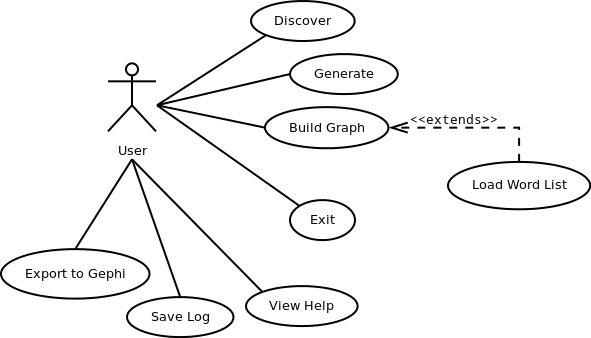
\includegraphics[scale=0.8]{WordPlay_UseCase}

Above is a UML use case diagram for this project. For the most part,
this diagram is self explanatory, however there are a few key points
that I would like to clarify. The word list extends from the build
graph scenario because the user may want to build or rebuild the graph
when the list of words may not already be loaded from a file. In this
case, the file must be loaded first. The scenario of being able to
``export to Gephi'' is that I plan to add the functionality to export
the graph data structure as a XML file readable by the Gephi graph
visualization program. This will be useful during the development
and testing of the application (to ensure I really have found a shortest
path) as well as a useful novelty. The save log feature would also
be able to allow the user to output the log generated by the proposed
GUI to be saved to file.


\subsection{UML Class Diagram}

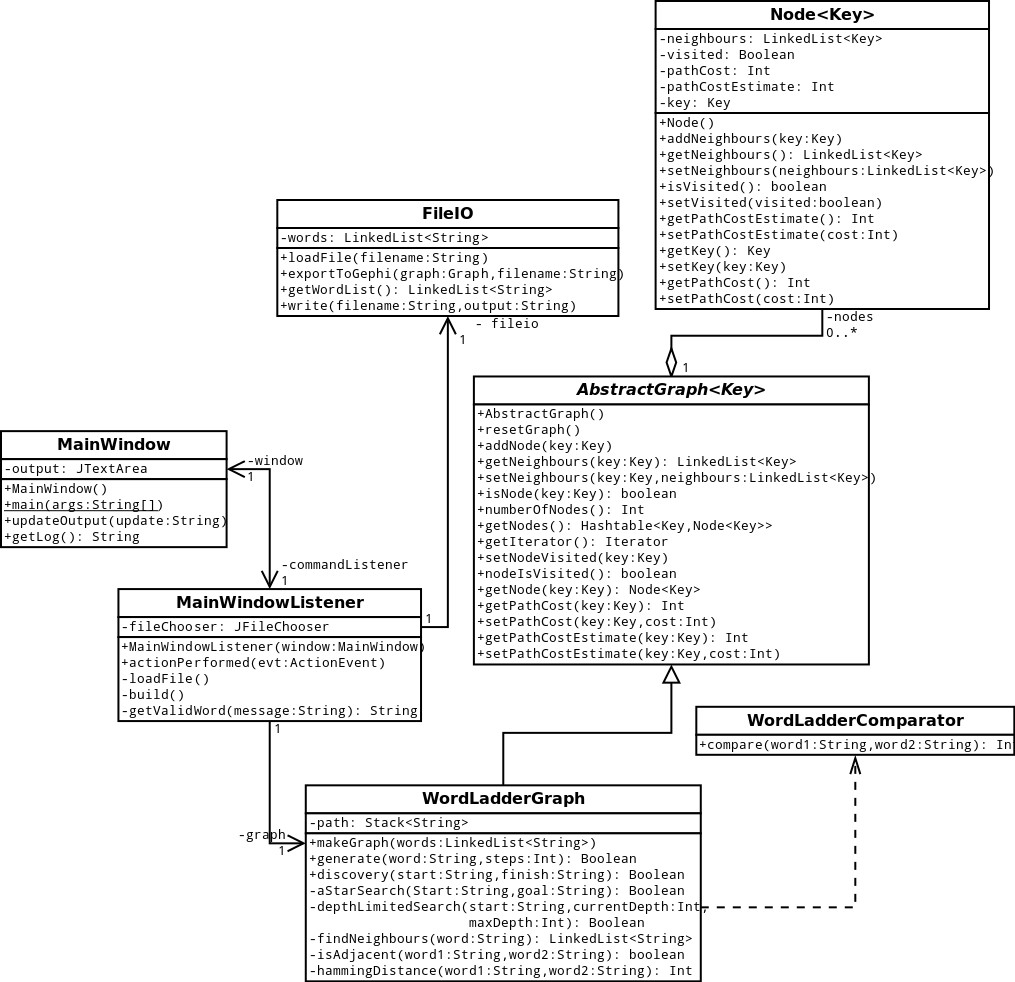
\includegraphics[scale=0.45]{WordPlay_UML}


\subsubsection{Description of the class diagram}
\begin{itemize}
\item \textbf{Main Window} - The main window class is the main JFrame window
for the application's GUI, as well as being the main entry point for
the program. The purpose of this class is simply to build the components
of the main window, assign them a listener object and deal with displaying
the GUI to the user. I have added a couple of additional methods to
this class which are used by the main window listener class. The update
output method is used to append text to the program log in the main
window. The get log method is used to get a contents of the program
log so that the main window listener can pass it to the file IO class
for exporting. 
\item \textbf{MainWindowListener }- The main window listener responds to
all events created by the main window of the application. This includes
loading a word file, building a graph object, exporting data to files
etc. This class is also responsible for checking that what the user
inputs is valid and that the user cannot do something illogical (such
as traverse a graph before it has been built). 
\item \textbf{FileIO} - The file IO class is responsible for getting and
outputting data to and from the file system. Functions of this class
include loading a list of words of an equal number of characters into
the program, writing the output of the GUI log to a file and exporting
a graph object into an XML format compatible with the Gephi graph
visualization program. This last function will come in handy when
developing the graph traversal algorithms, as I will be able to use
Gephi to check that my algorithm correctly identifies shortest paths
and handles unconnected graphs.
\item \textbf{AbstractGraph} - The abstract graph class is the most important
class in this design. It is a data structure which is designed to
represent a graph consisting of nodes and edges. The internal design
for the representation of a graph uses an adjacency list\cite{aho+hopcroft+ullman}
implemented using a hashtable of all the keys to the nodes in the
graph along with a node object which contains a list of this keys
to other nodes in the graph. I have designed this class to use a generic
for the key type of the hashtable as I want to make this class as
flexible and reusable as possible. In the case of our problem, I will
be using strings as the key. This class will also contain methods
for accessing nodes stored within the graph object, so that the user
does not have to call the get node method every time they wish to
access some node data.
\item \textbf{WordLadderGraph }- This class is where most of the major graph
manipulation occurs. The word ladder graph class is the implementation
point for creating and traversing the graph data structure. The two
major functions required in the problem description (word ladder generation
and discovery) will be implemented in this class. In order to traverse
the graph, it is planned that these operations will require the implementation
of a depth-limited search for generation and A{*} search for discovery
(see \subref{Algorithms}). This class also contains the make graph
method which builds a graph out of the list of loaded words. Note
that the search algorithms in this class will return a stack of nodes
representing the path, as they both work backwards from the goal node.
Therefore all nodes should be in the right order with the top element
representing the first node in the path.
\item \textbf{Node }- The node class is used to represent a single node
(vertex) within the graph data structure. This contains data about
the node (such as it's key, path cost and distance-cost estimate data
during a given traversal of the graph) as well a linked list of the
neighbors connected to this particular node. I have designed this
class to also use a generic type for the keys stored. This again makes
Graph/Node system more reusable as they do not necessarily have to
use a String as a key in a different implementation situation.
\end{itemize}

\subsection{Justification of Data Structures}

There are two key data structures that I plan to use to implement
in my design to solve the given problem. The first data structure
is a hashtable. For my solution I will be using the hashtable data
structure that comes supplied with the Java standard library. As mentioned
in the preceding section, I plan to use a hashtable to store string
variable as a key and a node object as the value for that key. My
justification for using a hashtable is that I want to be able to quickly
lookup words to find information stored at their associated node.
Using a hashtable is therefore quicker for this purpose as we do not
have to potentially iterate through the graph every time we wish to
access a node.

My reason for having a node object as the entry value of the hashtable
rather than simply having a linked list of neighbor nodes (as in the
basic implementation of an adjacency list) is that the node object
provides a convenient place to store data about this particular node,
other than simply listing it's neighbors. In my implementation, this
allows me to store whether the node has been visited during a given
traversal of the graph, its key and path cost data, but could be used
in future implementations to store other types of data as easily as
extending the node class.

The adjacency list data structure represented by both the abstract
graph and node classes provide an elegant and easily implemented solution
to the problem of representing the graph structure that will be generated
from a given input file of words. However, this graph/node data structure
implementation is designed to have low coupling with the rest of the
system, meaning that it can easily be lifted from this project and
reused in future development.

The graph/node pair also exhibits high cohesion. Both of these classes
only contain methods used for building and accessing data in the graph
structure, but will not implement any details regarding the rules
about how the graph structure should be built or how it should be
traversed, as these functions differ depending upon the intended use
of the graph. In this system, these details are instead delegated
to the concrete word ladder graph class which will actually build
the graph and implement the specific search algorithms required to
solve the given word ladder problems. One downside to this approach
is that the node and abstract graph classes exhibit high coupling
between each other. However, seeing as they are jointly supposed to
represent a single data structure (a graph), I feel that this is a
permissible exception as they are mainly designed to work in unison.

In conclusion, I believe that my design for the system represents
a simple and efficient way of internally representing the data required
by the application to solve the word ladder problem. I also feel that
this structure should allow me to create a system that exhibits principals
of both high cohesion and low coupling, as the underlying data structure
could be lifted directly out of this program and applied to future
programs with ease. Furthermore, I feel that this design could easily
be extended further. The abstract graph class could easily be used
as the basis for both directed and undirected graphs and the node
class could be extended to add any extra data or functionality that
a given problem might require beyond the scope of this program.


\subsection{Algorithms\label{sub:Algorithms}}

This section outlines the algorithms which I intend to use as part
of my solution to the word ladders problem. My choice of algorithms
to traverse the graph was to use a depth-limited search for the generation
of word ladders, and to use an A{*} search for the discovery of nodes
from a start point to a goal point. What follows is a pseudo code
listing of the algorithms that I plan to use to traverse the graph
data structure.

\noindent Listing 1 shows the pseudo code for the generation part
of my algorithm. This simply runs an instance of the depth-limited
search algorithm, but without a target node. This means that it will
go as deep into the graph as quickly as possible, until it reaches
the target depth or fails to find a path of the given depth. The generation
function will return an empty path if the desired number of steps
could not be reached.

\begin{lstlisting}[caption={Word Ladder generation function.},language=Java,numbers=left,showstringspaces=false,tabsize=4]
function generate(word, depth) {
	path = empty stack;
	result = depthLimitedSearch(word, 0, depth);

	if (result is a solution) {
		path = push word;
	} else (path size is less than desired steps) {
		path = empty stack;
	}
	
	reset distances in graph;
	return path;
}
\end{lstlisting}


The next pseudo code listing in this section shows the real guts of
the algorithm I propose to use to solve the generation problem. This
is a modified implementation for the recursive function for a depth-limited
search algorithm as described in AI: a modern approach\cite{russell+norvig}.
The major modification being that this search can only return two
states: whether we succeeded or failed to generate a word ladder of
the target depth, as opposed to Russell and Norvig's three states
(solution found, failed and cutoff).

\begin{lstlisting}[caption={Depth-Limited search algorithm used in generation mode.},extendedchars=true,language=Java,numbers=left,showstringspaces=false,tabsize=4]
function depthLimitedSearch(word, depth, maxdepth) {
	result = failed;	
	if(word not visited) {
		set word visited;
	}
	if(depth equal to maxdepth-1) {
		result = success;
	} else {
		while (word has neighbors && result is failure) {
			if(neighbor not visited) { 				
				result = depthLimitedSearch(neighbor, (currentDepth+1), maxdepth);
				if(result is success){
					push child onto path stack;					
				} 				
			} 			
		} 		
	} 	
	return result;
}	
\end{lstlisting}


The next two listings are for the discovery function which will use
an A{*} search to find the shortest path between two nodes in the
graph. The proposed A{*} search algorithm outlined below will take
into account the distance traveled into the graph as the path cost.
For it's heuristic, it will use the Hamming distance between the node
current being looked at and the goal node. The first listing shown
below is the function which will be used to initiate the breadth-first
search.

\begin{lstlisting}[caption={Word Ladder discovery function.},language=Java,numbers=left,showstringspaces=false,tabsize=4]
function discovery(start, finish){	
	path = empty stack;		
	result = breadthFirstSearch(start, finish); 	

	if(result is not success) { 			
		path = empty stack; 		
	}

	return path;
}
\end{lstlisting}


Finally, Listing 4 shows the proposed algorithm that will be implemented
in the A{*} search function. Including the building the solution path
back through the graph to the start node as done in the classic implementation
of Dijkstra's algorithm.

\begin{lstlisting}[caption={A{*} search algorithm used in discovery mode.},language=Java,numbers=left,showstringspaces=false,tabsize=4]
function aStarSearch(start, goal) {	
	result = failed;
	frontier = empty priority queue; 	
	previous = empty hashtable;	

	enqueue start to frontier;
	set pathcost(start) = 0;
	set distance-cost estimate(start) = 0 + hamming-distance(start);

	while (frontier has items && result is not success) { 			
		node = dequeue frontier;
		if(node is goal) { 				
			result = success; 		
		} else {
			tentative_path_cost = get pathcost(node) + 1;
			for(every child of node){
				if((child is not visited 
					OR tentative_path_cost <= pathcost(child)
					OR pathcost(child) not set)
					AND frontier does not contain child){
					
					set child as visited;
					set pathcost(child) = tentative_path_cost;
					set distance-cost estimate(child)
						= tentative_path_cost + hamming-distance(child, goal);

					enqueue child in frontier;
					add entry to previous (key=child, value=node);
				}		
			}	
		}	
	}

	if(result is success) {
		current=goal;
		while(current is not start) {
			current = get previous (key=current);
			push curren to path;		
		} 		
	}

	return result;
\end{lstlisting}



\subsection{Justification of Algorithms}

In order to solve the problems outlined in the brief for this assignment,
I have had to research two different approaches to traversing a graph.
In doing this I considered each option that was available and compared
each its advantages and disadvantages against the other available
options and the problem definition. In this section I justify why
I chose to use a depth-limited search for generation and A{*} search
for discovery.

I chose to use a depth-limited search for generation because the task
of generating a word ladder basically requires the program to traverse
through the graph by going as deep as possible (up to the required
number of steps to generate), as quickly as possible. The specification
only requires that we generate set of unique words from the given
word. The depth-limited search works taking the stating node and getting
all of it's neighbors. It then checks its neighbors for the first
unexplored node and then expands it, at which point the program repeats
itself. Going depth first allows us to generate as many unique nodes
as quickly as possible, seeing as the goal of generation is not to
find an especially shallow solution.

However my algorithm is modified from the standard implementation
for a depth-limited search as it does not have a ``target'' to search
for. Instead when the program reaches the limit point of the search,
this means we have managed to traverse the desired number of words
in the graph and hence a solution has been found. Therefore in my
implementation, where the program would normally hit the limit and
return that the search failed, it instead returns that the search
was successful. At this point, as the search ascends back up through
the recursive method calls, the algorithm pushes each of the current
nodes onto a stack so that when it reaches the top each of the nodes
in the path are in the correct order.

For the discovery mode of the program I have used a different search
technique to find the target goal. In order to find a path between
two nodes in the graph, the program needs to implement a shortest
path search algorithm. The depth-limited search is not appropriate
for this problem because it is not guaranteed to find an optimal solution
(as it evaluates deeper nodes first). Also, because of the depth limit,
it is not guaranteed that to even find a solution!

Clearly a different approach must be taken to solve this problem.
Instead, I researched a variety of different search options to find
the shortest path between the two nodes. Initially I started looking
at uninformed search techniques. Of the main uninformed search techniques,
the solutions which proved to be the most appropriate the the problem
at hand were breadth-first search (with the path building technique
outlined in Dijkstra's algorithm) and iterative deepening depth-first
search. Both of these options proved to be acceptable options which
would be able to find optimum and complete solutions in a reasonable
amount of time.

However, I realized that my function for checking if two strings are
adjacent could provide additional information that could be of use
to the program. This function calculated the Hamming distance of two
nodes, which is the numerical letter difference between two strings.
I realized that this could potentially be used as a heuristic to guide
an informed search algorithm to a specified goal, much in the same
way that an n-puzzle can be solved quicker by using Manhattan distances
as the heuristic. This heuristic is also guaranteed to be admissible
no matter what the word, as the Hamming distance between any given
word and the goal word can never be more than the optimal path. This
means that this particular heuristic will provide us with both an
optimal and complete solution, assuming one exists.

I therefore chose to use the A{*} search algorithm for discovery mode,
as this generally the most effective informed search technique; considering
both path cost and a heuristic estimate. My implementation uses the
Java standard library priority queue with a comparable object that
I created myself. The comparable object is used to compare the distance-cost
estimate (that is the cost of the current path, plus the Hamming distance
of the current node) and calculate the difference. The node with the
lowest score in the list then has the greatest priority and is subsequently
chosen first. The algorithm then proceeds to examine each applicable
child node, calculating its path cost from the start node (simply
an increase of one for every edge traversed) and calculating the Hamming
distance for the current word. As the algorithm adds children to the
queue, it also records a link back to the parent node so that we can
rebuild the path back from the goal to the start node.

I feel that the A{*} search algorithm is a justified choice for finding
the shortest path between two nodes in our graph. In the worst case
scenario, where the start and goal nodes are part of unconnected graphs
or are connected by a very long path, the search algorithm will behave
much like a breadth-first search and no additional benefit will occur.
As I was initially planning to use breadth-first search, there is
effectively no real loss to the time required to traverse the graph,
even in the worst case scenario. But when the heuristic kicks in as
the algorithm finds a node seemingly closer to the goal, there will
be a noticeable reduction in the number of nodes that the algorithm
has to examine in order to reach the target. Simply compare the results
of finding a path from the word ``head'' to the word ``foot'';
Breadth-first search will examine 499 nodes before finding an optimal
path of six nodes, while A{*} will find a six node path by examining
only 26 nodes.


\section{Testing}

This part of the document outlines the testing of the application.
It is split into three parts: JUnit testing, Input testing (ensuring
that correct results are found in discovery/generation) and testing
the GUI.


\subsection{JUnit Testing}

During the development of this application I have been using JUnit
test cases as a quick fire way to check that the systems classes are
working as expected. This was particularly useful when it came to
ensuring that the generate and discovery modes were working properly
as I could check that they were returning valid results without having
to load the GUI part of the application or manually load the dictionary
file. The full set of JUnit tests are supplied with the deliverables
for this assignment and can be found in the tests package.


\subsection{Input Testing}

In this section, I use a selection of testing data to check that the
algorithms for generation and discovery are able to create correct
and valid word ladders. I provide both a test table of the data used
and screen shot evidence of each test being carried out using the
GUI for this application.


\subsubsection{Input Test Table}

\begin{tabular}{|>{\raggedright}p{0.02\textwidth}|>{\raggedright}p{0.1\paperwidth}|>{\raggedright}p{0.15\textwidth}|>{\raggedright}p{0.15\textwidth}|>{\raggedright}p{0.15\textwidth}|>{\raggedright}p{0.15\textwidth}|}
\hline 
\# & Mode: (Gen/Dis) & Input & Expected Outcome & Actual Outcome & Comment\tabularnewline
\hline 
\hline 
1 & Generate & Word = ``hold'';

Steps = 10 & hold, held, meld, mend, tend, tent, text, test, teat, feat & As expected & \tabularnewline
\hline 
2 & Generate & Word = ``ha''

Steps = 3 & ha, ma, my & As expected & \tabularnewline
\hline 
3 & Generate & Word = ``how''

Steps = 5 & how, tow, toy, tot, tor & As expected & \tabularnewline
\hline 
4 & Generate & Word = ``head''

Steps = 2346 & Unable to find path. & As expected. & Number of steps was greater than the number of nodes in the graph.\tabularnewline
\hline 
5 & Generate & Word = ``head''

Steps = 1000 & head, mead, mend, ..., crew, craw & As expected. & \tabularnewline
\hline 
6 & Discovery & Start = ``head''; 

Goal = ``foot'' & 6 node path; 

head, bead, beat, boat, boot, foot & As expected & \tabularnewline
\hline 
7 & Discovery & Start = ``me''; 

Goal = ``do'' & 4 node path; 

me, he, ho, do & As expected & \tabularnewline
\hline 
8 & Discovery & Start = ``fight''; 

Goal = ``deals'' & Unable to find path. & As expected & ``Fight'' and ``deals'' are unconnected nodes\tabularnewline
\hline 
9 & Discovery & Start = ``bin''

Goal = ``bed'' & 3 node path;

bin, bid, bed & As expected. & \tabularnewline
\hline 
10 & Discovery & Start = ``tub''

Goal = ``hub'' & 2 node path;

tub, hub & As expected. & \tabularnewline
\hline 
11 & Discovery & Start = ``big''

Goal = ``big'' & 1 node path;

big & As expected. & \tabularnewline
\hline 
\end{tabular}


\subsubsection{Screen Shot Evidence of Testing}

Screen shot \#1

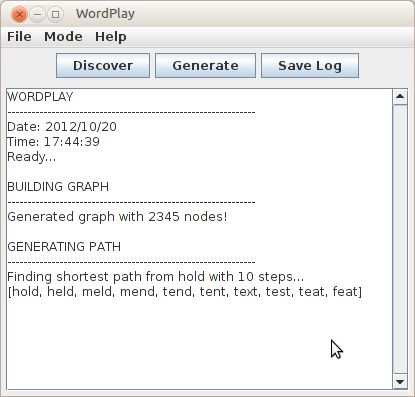
\includegraphics[scale=0.5]{screen-shot1}

Screen shot \#2

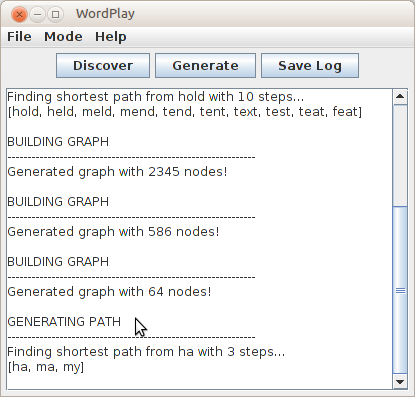
\includegraphics[scale=0.5]{screen-shot2}

Screen shot \#3

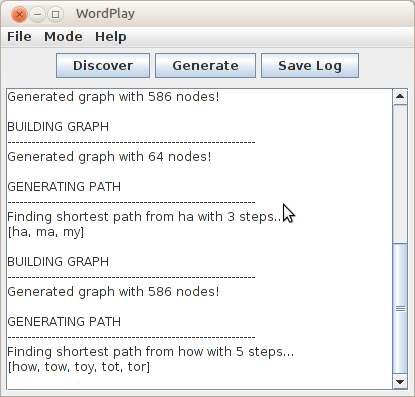
\includegraphics[scale=0.5]{screen-shot3}

Screen shot \#4

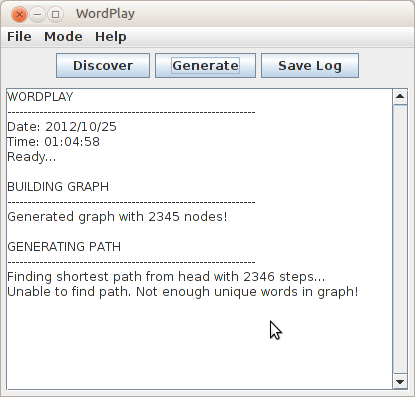
\includegraphics[scale=0.5]{pasted4}

Screen shot \#5

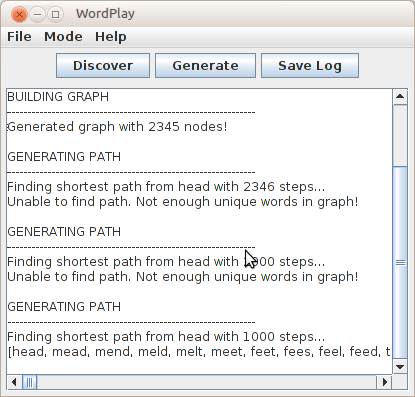
\includegraphics[scale=0.5]{screen-shot5}

Screen shot \#6

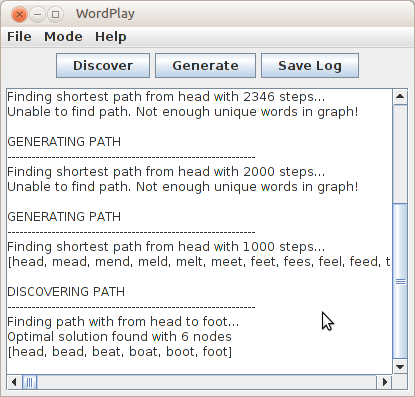
\includegraphics[scale=0.5]{screen-shot6}

Screen shot \#7

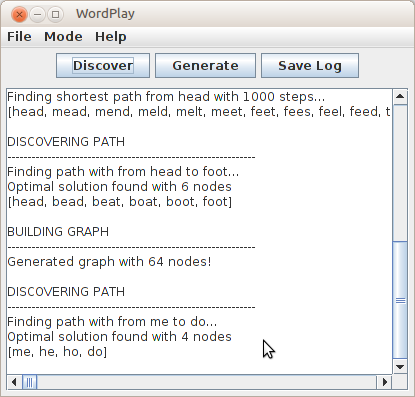
\includegraphics[scale=0.5]{screen-shot7}

Screen shot \#8

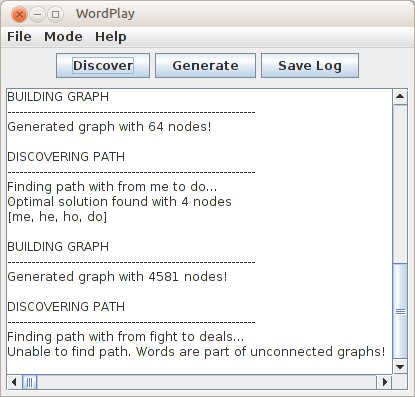
\includegraphics[scale=0.5]{screen-shot8}

Screen shot \#9

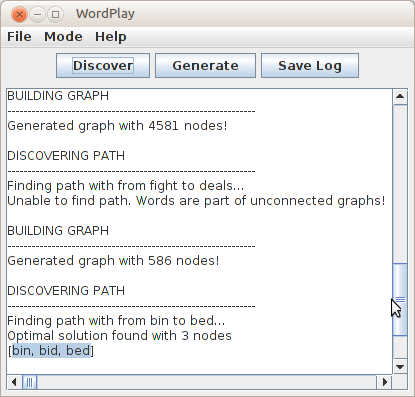
\includegraphics[scale=0.5]{screen-shot9}

Screen shot \#10

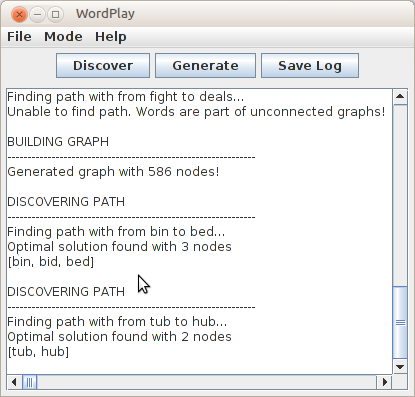
\includegraphics[scale=0.5]{screen-shot10}

Screen shot \#11

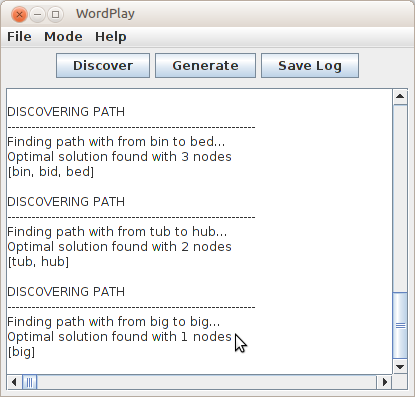
\includegraphics[scale=0.5]{screen-shot11}


\subsection{GUI Testing}

\begin{longtable}{|c|>{\raggedright}p{0.17\textwidth}|>{\raggedright}p{0.17\textwidth}|>{\raggedright}p{0.17\textwidth}|>{\raggedright}p{0.17\textwidth}|>{\raggedright}p{0.17\textwidth}|}
\hline 
\# & Testing & Data & Expected & Actual & Comment\tabularnewline
\hline 
\hline 
1 & Build Graph & Select build graph option. Choose ``dict4.dat'' file. & File chooser shown. Selected file is built into graph. Output is updated
with confirmation. & As expected. & \tabularnewline
\hline 
2 & Build Graph & Select build graph option. Select cancel. & File chooser should exit back to main window. & No input file loaded dialog shown. & Logical window showing error. Fixed.\tabularnewline
\hline 
3 & Rebuild Graph & Select rebuild graph. Load file when prompted asked. & No input file dialog shown. Should then be able to load file and build
graph. & As expected. & \tabularnewline
\hline 
4 & Rebuild Graph & Select rebuild graph. Cancel when prompted to load file. & Dialog should exit back to main window. & As expected. & \tabularnewline
\hline 
5 & Rebuild Graph & Build a graph, then select rebuild graph. & Should remake the graph and output results to text area. & As expected. & \tabularnewline
\hline 
6 & Save Log & Select save log. & Prompted from file name. Output is saved to file. & As expected. & \tabularnewline
\hline 
7 & Save Log & Select save log. Click cancel when prompted for name. & Prompt exist back to main window. & Failed. NullPointerException thrown. & No check for empty input. Fixed.\tabularnewline
\hline 
8 & Export to Gephi & Select export to Gephi without building graph. & Warning that the graph hasn't been built should be shown. & As expected. & \tabularnewline
\hline 
9 & Export to Gephi & Build a graph then select export to Gephi. & Prompted for name of output file. Graph exported to file. & As expected. & \tabularnewline
\hline 
10 & Export to Gephi & Build a graph then select export, click cancel when prompted for filename & Prompt exits back to main window & Failed. Exports graph to ``null.gexf'' & No check for empty input. Fixed.\tabularnewline
\hline 
11 & Generate & Click generate when no graph is built & Warning that no graph is built shown & As expected. & \tabularnewline
\hline 
12 & Generate & Build graph. Run generate mode with values:

word = ``hold''

steps = 10 & 10 steps should be generated starting with the word hold. & As expected. & \tabularnewline
\hline 
13 & Generate & Build graph. Run generate but cancel on first prompt. & Prompt exits back to main window. & Failed. That wasn't a number exception shown. & Program continued even if user clicks cancel on prompt. Fixed.\tabularnewline
\hline 
14 & Generate & Build graph. Run generate but cancel on second prompt & Prompt exits back to main window. & Failed. Invalid number exception thrown & Program reads in null instead of a string. Fixed\tabularnewline
\hline 
15 & Generate & Input invalid word. 

word = ``hello'' & Error message shown. & As expected. & \tabularnewline
\hline 
16 & Generate & Input letters instead of a number.

steps = ``hi'' & Error Message shown & As expected. & \tabularnewline
\hline 
17 & Discovery & Click discovery when no graph is built. & Warning that no graph is built shown & As expected. & \tabularnewline
\hline 
18 & Discovery & Build graph. Run discovery but cancel on first prompt. & Prompt exits back to main window. & As expected. & \tabularnewline
\hline 
19 & Discovery & Build graph. Run discovery, but cancel on second prompt & Prompt exits back to main window. & As expected. & \tabularnewline
\hline 
20 & Discovery & Input an invalid word for the first prompt

word = ``hello'' & Error message shown. & As expected. & \tabularnewline
\hline 
21 & Discovery & Input an invalid word for the second prompt

word = ``hi'' & Error message shown. & As expected. & \tabularnewline
\hline 
22 & Discovery & Input valid words

start = ``hold''

goal = ``jack'' & Output updated with correct path from both nodes. & As expected. & \tabularnewline
\hline 
23 & About Dialog & Click about option from menu. & About menu shown. & As expected. & \tabularnewline
\hline 
24 & Exit & Click exit option from menu. & Program exits & As expected. & \tabularnewline
\hline 
\end{longtable}

\bibliographystyle{plain}
\bibliography{refs}


\appendix

\section*{Source Code Listing}

The rest of this document provides a full print out of the final Java
source code that makes up my application. Full Javadoc and a runnable
jar file have also been submitted with the electronic copy of the
assignment. All of the code provided here has been complied and run
from the command line on both Ubuntu 12.04 and a standard Windows
7 machine in B23.
\end{document}
